\chapter{Discussion
  \label{chap:discussion}}

\section{Column density and Rotation temperature}

In this subsection we will describe the methodologies in deriving the column density and the rotational temperature of COMs.
The column density of CH$_{3}$NH$_{2}$ ($N_{\mathrm{MA}}$) was estimated by using 
the rotational temperature diagram method, which assumes local thermodynamic equilibrium 
(LTE) and optically thin emission. 
The following equation was employed for the analysis \citep{Turner1991}:
\begin{align}
\log \dfrac{3\,k_{\mathrm{B}}\,T_{\mathrm{B}} \,\Delta V_{1/2}}{8\, \pi^3\, \nu\, S\, \mu_0^2} = \log \dfrac{N_{\mathrm{MA}}}{U_{\mathrm{rot}}} - \dfrac{E_{\mathrm{u}}}{k_{\mathrm{B}}} \dfrac{\log e}{T_{\mathrm{rot}}}
\label{eq:RD}
\end{align}

In the expression, $\nu$ is the rest frequency of the transition, $\mu_0$ is the permanent dipole moment, 
$U_{\mathrm{rot}}$ is the rotational partition function, $S$ is the line strength, 
$E_{\mathrm{u}}$ is the upper state energy, and $ T_{\mathrm{B}}$ and  $\Delta V_{1/2}$ 
are the brightness temperature and line widths (FWHM, in~km~s$^{-1}$), respectively.
We assumed the average $\Delta V_{1/2} = 4.2\, \mathrm{km\,s^{-1}}$, which derived by the Gaussian fitting.

The brightness temperature can be converted from intensity $I_{\mathrm{\nu}}$
when the Rayleigh-Jeans law is applicable.
\begin{align}
T_{\mathrm{B}} = \dfrac{c^2}{2\,k_{\mathrm{B}}\, \nu^2} \,I_{\mathrm{\nu}}
\end{align}

\begin{figure}[H]
  \centering
  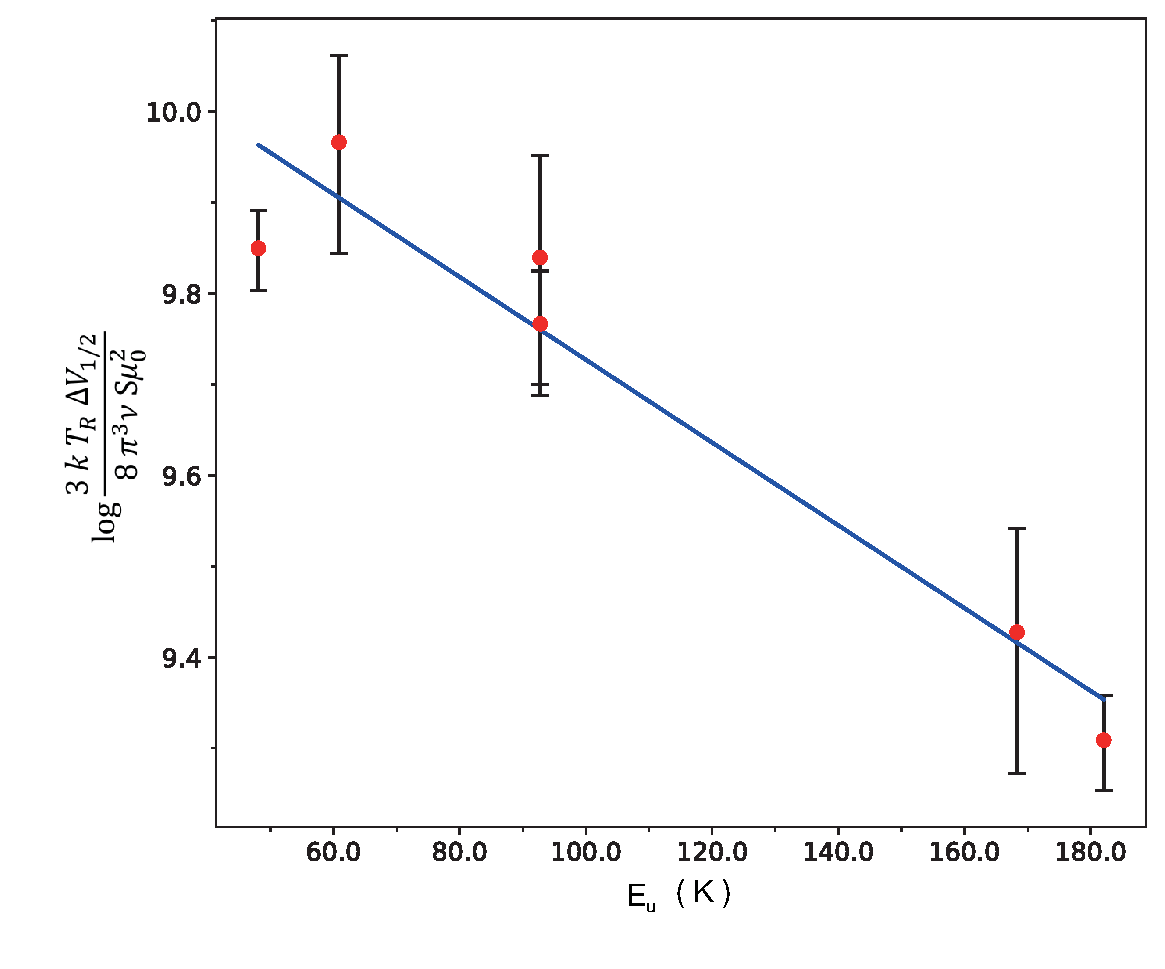
\includegraphics[width=0.8\textwidth]{OrionKL/RD_6point_label.eps}
  \caption{Rotation diagram of CH$_{3}$NH$_{2}$ in Hot core. The error bars represents $\pm$ 3 $\sigma$ for each data.}
  \label{fig:RD}
\end{figure}

The resulting plots are given in Figure \ref{fig:RD}.
The analysis yields a rotational temperature of $T_{\mathrm{rot}} =  95.4^{+15.5}_{-11.7} \,\,\mathrm{K}$, 
with a column density of $N_{\mathrm{MA}} = ( 5.5^{+1.6}_{-1.1} ) \times 10^{14} \,\,\mathrm{cm^{-2}}$.

\section{Suspicious lines}
Comparison of catalogs did not suggest contamination, but some emission lines could not be detected as CH$_{3}$NH$_{2}$.

\renewcommand{\arraystretch}{1.5}
\begin{table}[htb]
\begin{center}

  \caption{transitions of CH$_3$NH$_2$}
  \label{tab:unresolved}
{\scriptsize
  \begin{tabular}{ccccccccl} \hline
   Frequency & S$\mu ^{2}$ & E$_{\rm{u}}$& Transition & peak $T_{\mathrm{B}}$\footnotemark[1] & $V_{\mathrm{LSR}}$\footnotemark[1]  & Noise & Conversion  & Comments \\ 
  $\,$ [GHz]  & [D$^2$] &  [K] & ($J$, $K_{\rm{a}}$, $\Gamma$)  & [K] & [km s$^{-1}$] & [K] &  (K to Jy beam$^{-1}$) &  \\ \hline 
    215.670 & 53.92 & 111.48 & 9, 2, $E_{1-1}$ $\rightarrow$ 9, 1, $E_{1+1}$  & 3.74(0.07) & 5.37(0.07) & 0.043 & 0.077 &  \\
    221.755 & 35.06 & 133.11 & 10, 2, $A_{2}$ $\rightarrow$ 10, 1, $A_{1}$ & 0.33(0.03)& 5.35(0.19) & 0.133 &0.108 &SV data \\ \hline
  \end{tabular}
  }
\end{center}
\end{table}
\footnotetext[1]{Numbers in parenthesis represent standard deviation in the unit of the last significant digits.}


As shown in Figure \ref{fig:RD_blend}, the CH$_{3}$NH$_{2}$ data including 2 transitions in Table \ref{tab:unresolved} 
produced point-to-point scatter perhaps because of the lower signal-to-noise ratio for the weaker transitions in SV data 
and possible high-level contamination.

\begin{figure}[htp]
  \centering
  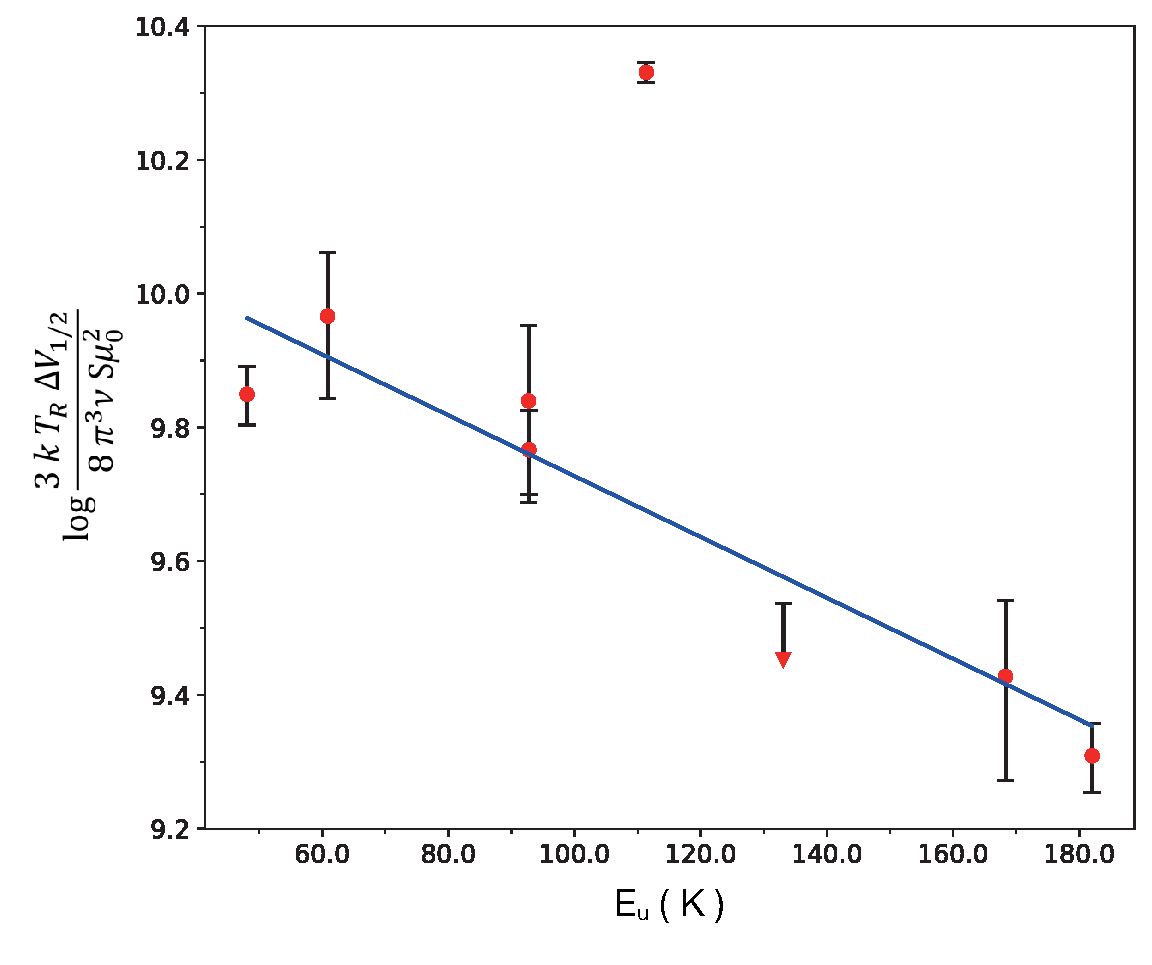
\includegraphics[width=0.7\textwidth]{OrionKL/RD_blend.eps}
  \caption{Rotation diagram of CH$_{3}$NH$_{2}$ in Hot core with additional 2 lines. The error bars on round plots represents $\pm$ 3$\sigma$ for each data. A signal below 3$\sigma$ is represented by a triangle with the error bar indicating the upper limit. The blue line is the same one as Figure \ref{fig:RD}.}
  \label{fig:RD_blend}
\end{figure}

\subsection*{215.670 GHz line}
This emission line ($E_{\mathrm{u}}=111$ K) is seen at Hot core and IRc7 like other CH$_{3}$NH$_{2}$ transitions 
(see Figure 4.3 and Figure \ref{ch_4}), but this line has stronger intensity than that predicted in the rotation diagram (see Figure \ref{fig:RD_blend}).
Since the line width is also wider than the other CH$_{3}$NH$_{2}$ transitions (see Figure 4.3), 
it appears that this line is blended with other molecular emission lines existing in Hot core.
Then examining the catalog including the transition of higher excitation, CH$_3$CH$_2$CN (215.6687 GHz, $E_{\mathrm{l}}$ = 604.845 K)
has come up as a candidate for blending.
However, considering that T$_{\mathrm{rot}}$ of CH$_3$CH$_2$CN in Hot core is 155 K \citep{Feng+2015}, 
it is uncertain how much this transition of higher excitation contributes to the blending.

\begin{figure}[htp] 
\begin{center}
\begin{minipage}{0.98\textwidth} 
\begin{center}
\begin{minipage}{0.48\textwidth}
\begin{center}
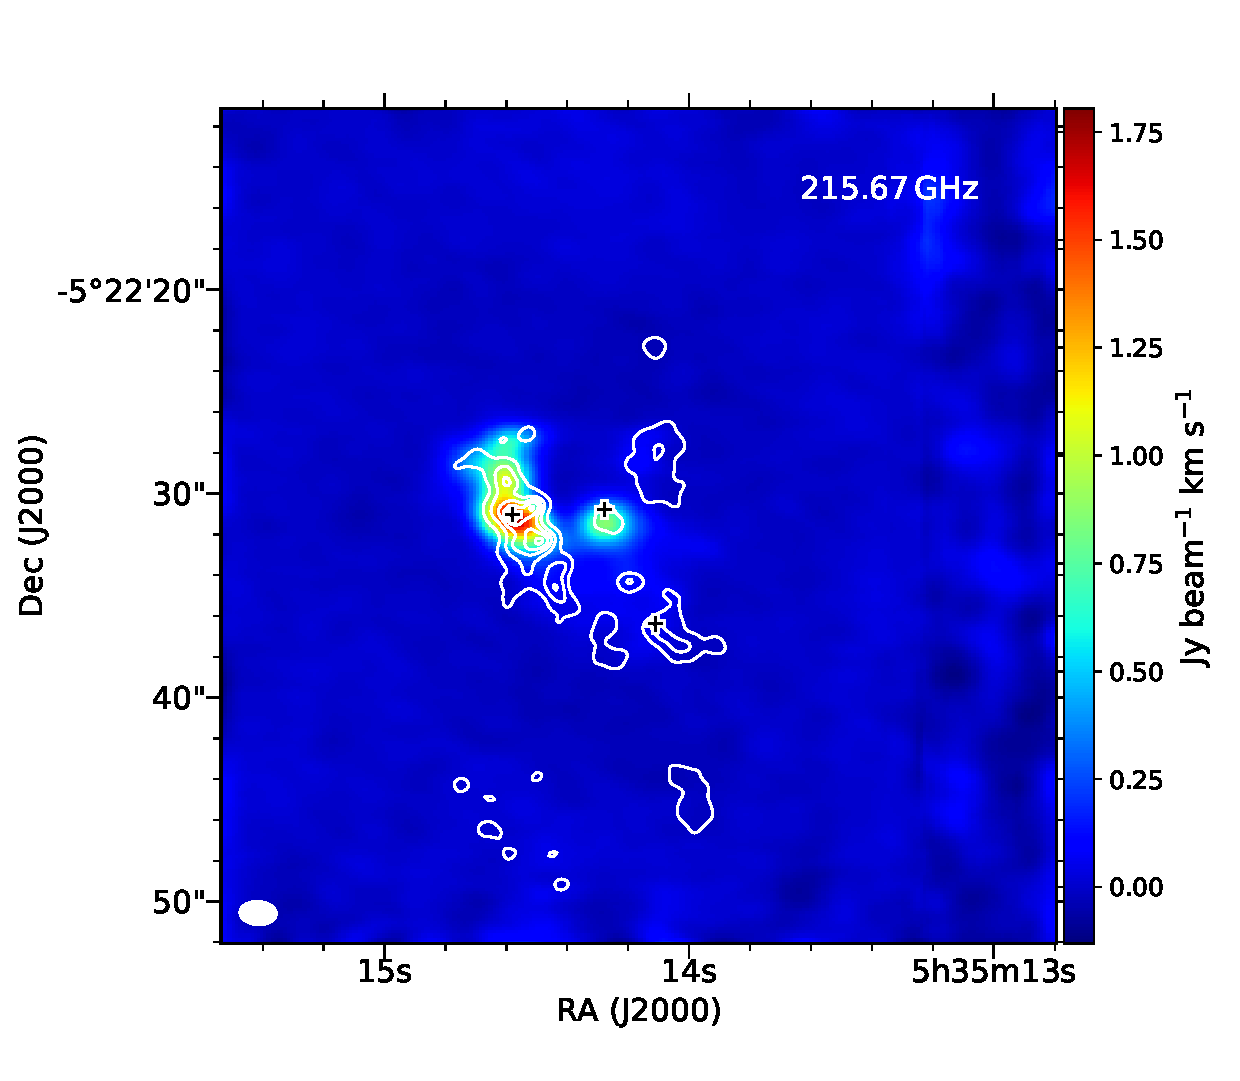
\includegraphics[width=0.98\textwidth]{OrionKL/mom0/215.67mom0_3-7.eps}
\end{center}
\end{minipage}
\begin{minipage}{0.48\textwidth}
\begin{center}
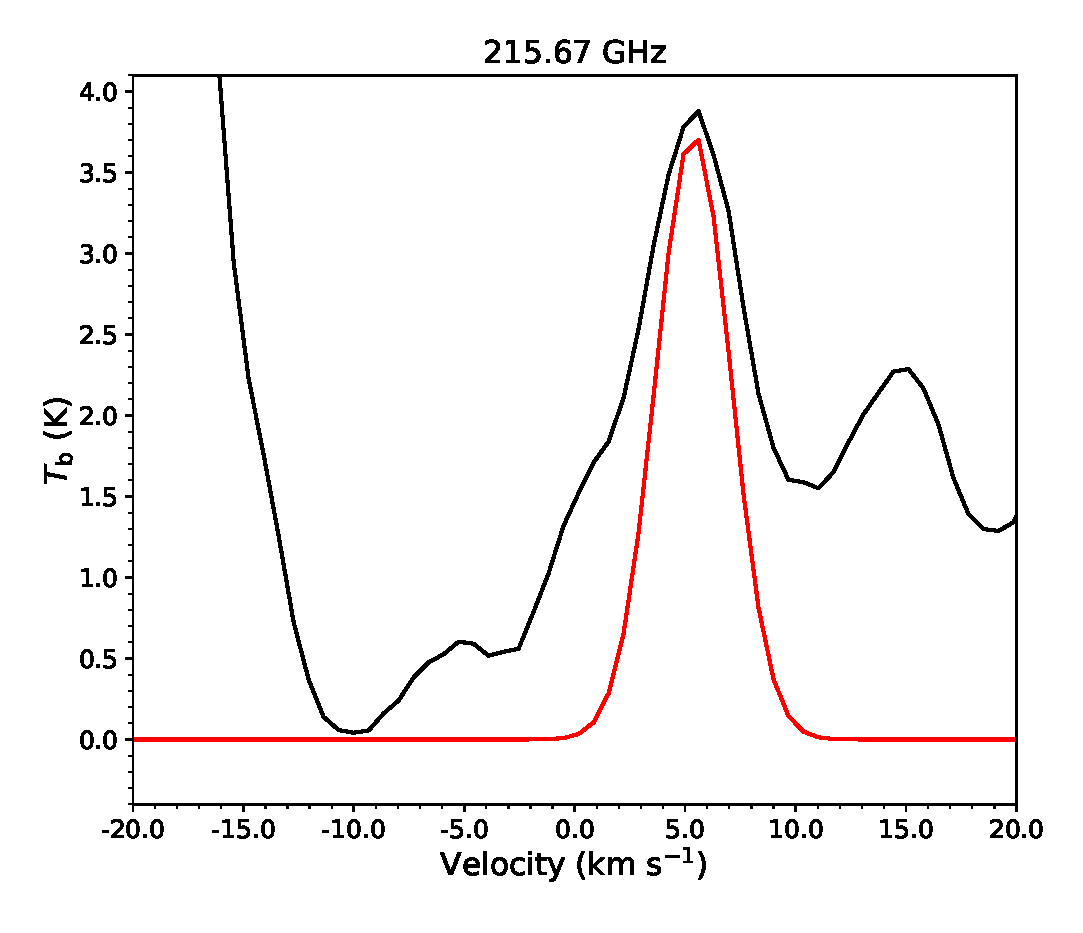
\includegraphics[width=0.98\textwidth]{OrionKL/spectrum/HC/215.6696452w_fit.eps}
\label{fig:215spec}
\end{center}
\end{minipage}
\end{center}
\end{minipage}
\label{fig:215data}
\caption{(left) Integrated intensity map of the emission for 215.670 GHz. Same as Figure \ref{fig:cont+2015} but for white contours and black crosses. (right) Spectrum of the CH$_3$NH$_2$ lines at each frequency observed in Hot core (black)  and the result of the Gaussian fitting assuming the average $\Delta V_{1/2} = 4.2\, \mathrm{km\,s^{-1}}$ (red)}
\end{center}
\label{fig:215data}
\end{figure}

\subsection*{221.755 GHz line}
A faint signal was seen in Hot core in the integrated intensity map and channel maps (Figure 4.4 and \ref{ch_6}).
Since there was no blend of other molecular emission lines in the comparison with the catalogs, we analyzed the spectrum, 
but the peak intensity ( $T_{\mathrm{B}}=$ 0.33 K) was weaker than 
3 $\sigma $ noise level ($T_{\mathrm{B}}=$ 0.133 K, see Table \ref{tab:unresolved}). 
When we plotted this line on the rotation diagram with 3$\sigma$ as the upper limit of the intensity, 
the derived value was consistent with other CH$_3$NH$_2$ transitions (see Figure \ref{fig:RD_blend}). 
This emission line was included in SV data cube, 
so it could be possible to detect the line in future observations with higher S/N ratio.

\begin{figure}[htp] 
\begin{center}
\begin{minipage}{0.98\textwidth} 
\begin{center}
\begin{minipage}{0.48\textwidth}
\begin{center}
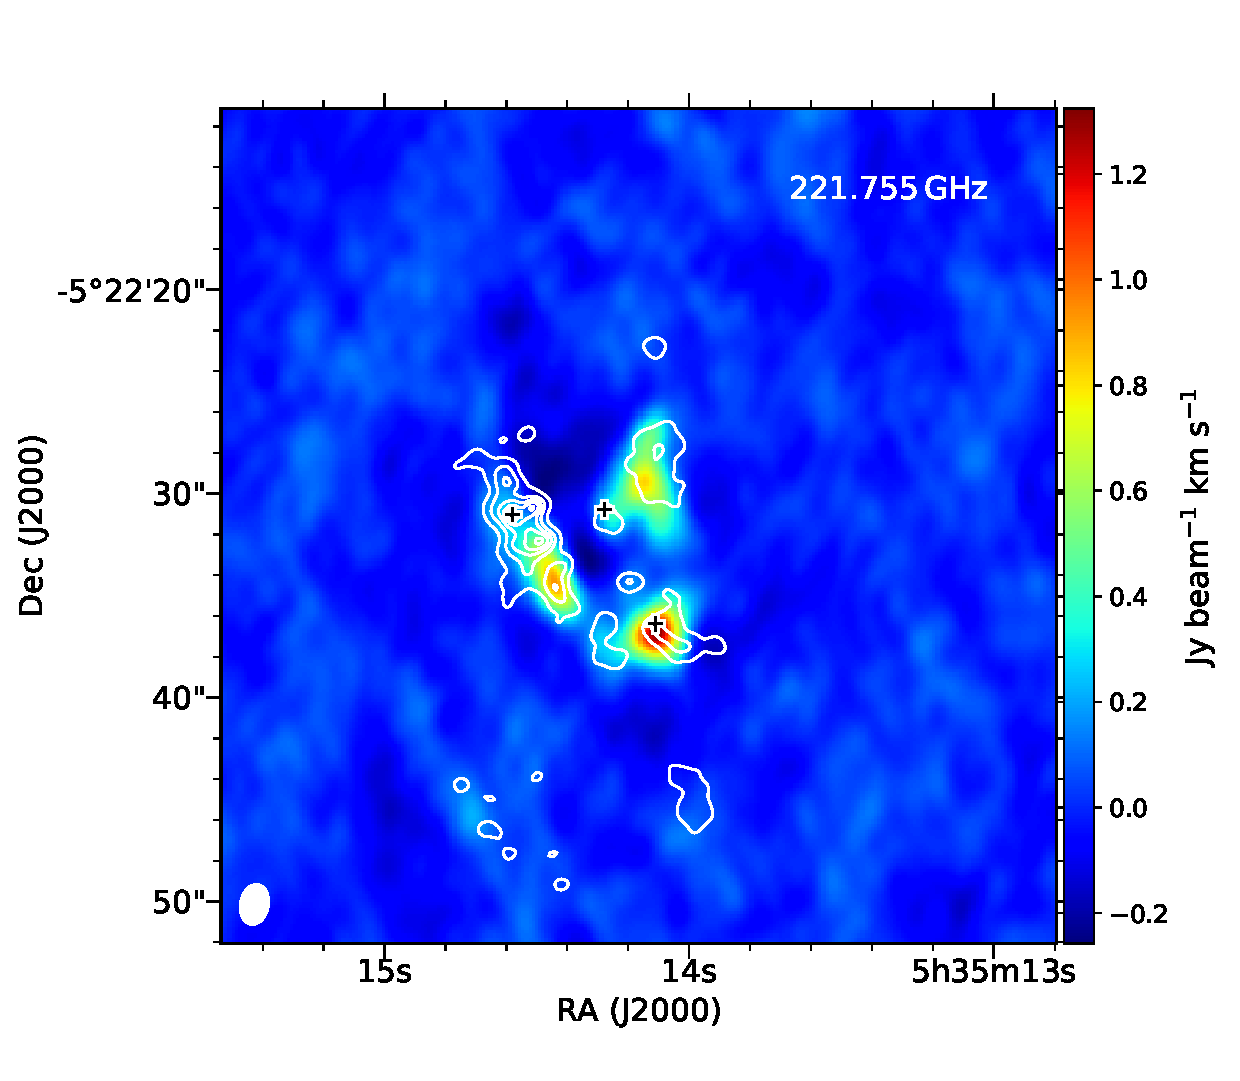
\includegraphics[width=0.98\textwidth]{OrionKL/mom0/221.755SV_mom0_3-7.eps}
\label{fig:221mom}
\end{center}
\end{minipage}
\begin{minipage}{0.48\textwidth}
\begin{center}
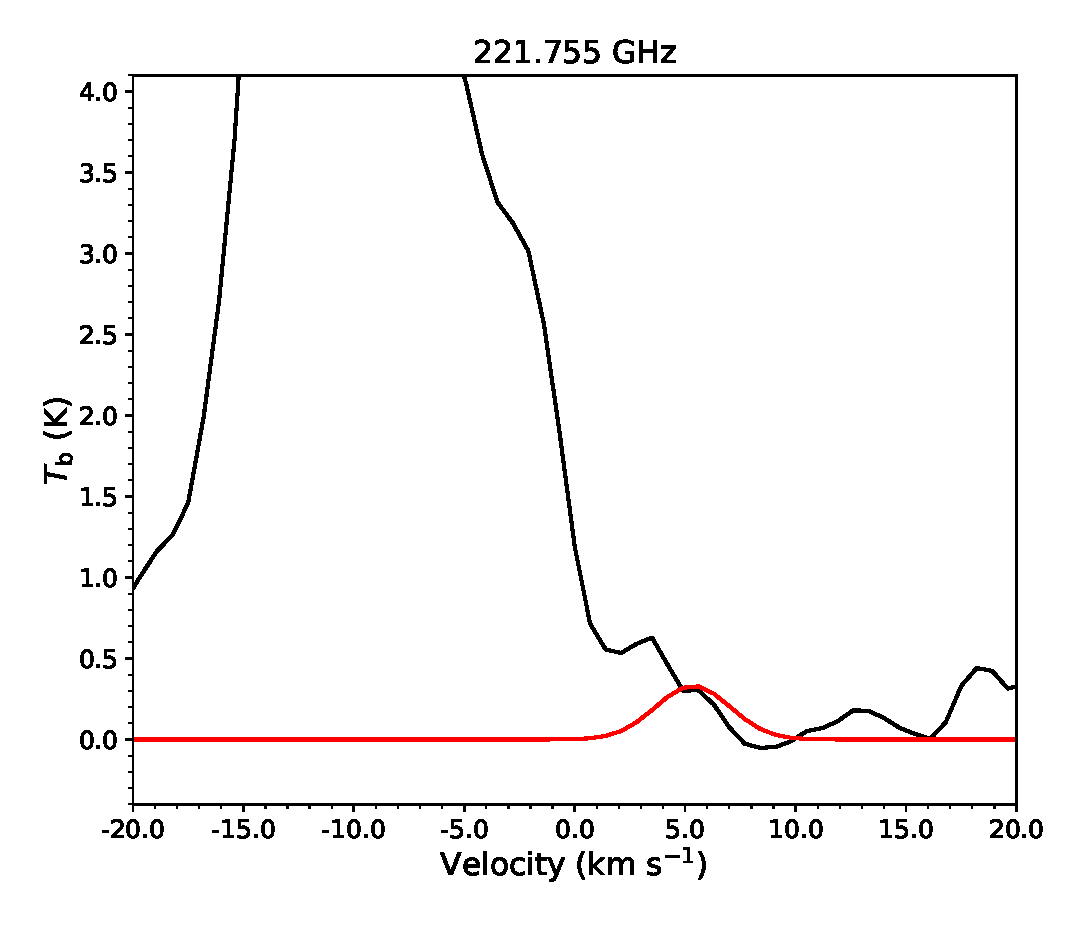
\includegraphics[width=0.98\textwidth]{OrionKL/spectrum/HC/221.755055w_fit.eps}
\end{center}
\end{minipage}
\end{center}
\end{minipage}
\caption{(left) Integrated intensity map of the emission for 221.755 GHz. Same as Figure \ref{fig:cont+2015} but for white contours and black crosses. (right) Spectrum of the CH$_3$NH$_2$ lines at each frequency observed in Hot core (black)  and the result of the Gaussian fitting assuming the average $\Delta V_{1/2} = 4.2\, \mathrm{km\,s^{-1}}$ (red)}
\end{center}
\end{figure}

\begin{figure}[htp]
  \centering
  \includegraphics[width=0.98\textwidth]{OrionKL/chmap/215.67.eps}
  \caption{Channel map around 215.670 GHz. Same as Figure \ref{ch_0} but for white contours and mazenta crosses.}
  \label{ch_4}
\end{figure}

\begin{figure}[htp]
  \centering
  \includegraphics[width=0.98\textwidth]{OrionKL/chmap/221.755.eps}
  \caption{Channel map around 221.755 GHz line. Same as Figure \ref{ch_0} but for white contours and mazenta crosses.}
  \label{ch_6}
\end{figure}
